\documentclass[russian]{beamer}

\usetheme{confposter}

\usepackage[size=a0,orientation=portrait,scale=1.6]{beamerposter}
\usepackage{units}
\usepackage{float}
\usepackage{subfig}
\usepackage{fontspec}
\usepackage{picture}
\usepackage{eso-pic}
\defaultfontfeatures{Ligatures=TeX}

\setmainfont{Times New Roman Cyr}
\setsansfont{Times New Roman Cyr}

\title{Временное растяжение ГэВ излучения гамма-всплесков:\\[0.2ex]Fermi LAT и геометическая модель}
\author{
	{\Large Максим Пискунов$^{*}$ и Григорий Рубцов} \\[0.5ex]
	{\large Институт ядерных исследований РАН} \\[0.4ex]
	{\large МГУ им. М.В. Ломоносова} \\[0.6ex]
	{\normalsize $^{*}$\href{mailto:maxit@ms2.inr.ac.ru}{maxit@ms2.inr.ac.ru}} \\
	\hfill {\normalsize \url{https://github.com/maxitg/GammaRays}}
}

\begin{document}
	
	\begin{frame}
		\begin{columns}[t]

			\begin{column}[t]{0.4\linewidth}

			   	\begin{block}{Введение}
					Наблюдения показывают, что излучение гамма-всплесков с энергией выше \unit[100]{МэВ} систематически наблюдается позже, чем низкоэнергичное излучение. Различия же кривых блеска в различных диапазонах высокоэнергичного (> \unit[100]{МэВ}) излучения изучены хуже. В данной работе мы изучаем различия кривых блеска в диапазонах (\unit[100]{МэВ}, \unit[1]{ГэВ}) и (\unit[1]{ГэВ}, \unit[300]{ГэВ}).
			   	\end{block}

			   	\begin{block}{Наблюдения}

					\begin{figure}

						\centering
						{\large Сравнение кривых блеска GRB 090926A (тест Колмогорова-Смирнова)}
						\subfloat{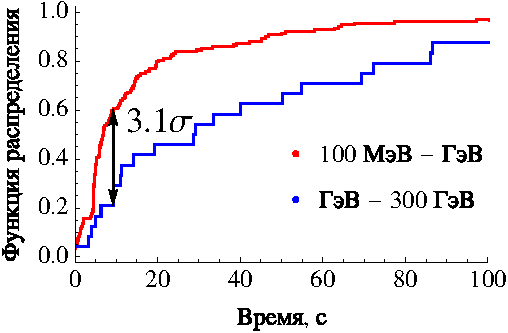
\includegraphics[width=\textwidth]{090926A.pdf}} \\
						\subfloat{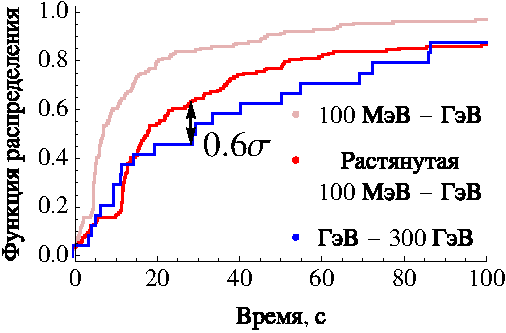
\includegraphics[width=\textwidth]{090926AStretched.pdf}} \\
						\label{Figures}

					\end{figure}

					\begin{itemize}
						\item{Рассмотрены 3 гамма-всплеска: 080916C, 090902B и 090926A.}
						\item{Кривые блеска 080916C и 090902B в рассматриваемых диапазонах совпадают в пределах $2\sigma$.}
						\item{Излучение 090926A в диапазоне (\unit[1]{ГэВ}, \unit[300]{ГэВ}) растянуто относительно менее энергичного со статистической значимостью $3.1\sigma$.}
					\end{itemize}

			   	\end{block}

			\end{column}

			\begin{column}[t]{0.4\linewidth}

			   	\begin{block}{Модель}

			   		\begin{figure}
						\centering
						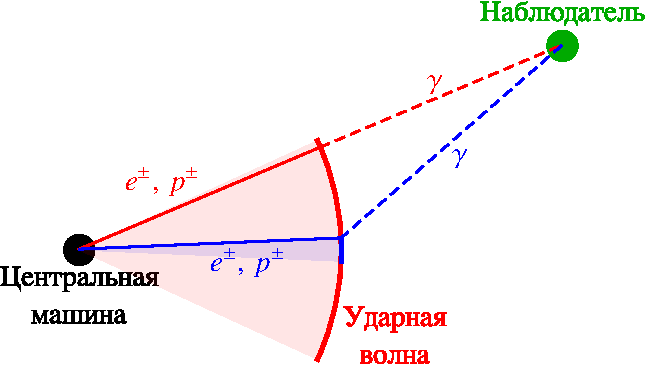
\includegraphics[width=\textwidth]{modelExplanation.pdf}
						\label{fig:modelExplanation}
			   		\end{figure}

					Мы предлагаем простую геометрическую модель, объясняющую временное растяжение. Основное предположение -- чем выше энергия излучения, тем ближе к оси джета оно излучается.

					\begin{enumerate}
						\item{В момент времени $t = 0$, центральная машина излучает сферическую ударную волну.}
						\item{Ударная волна распространяется с ультрарелятивистской скоростью.}
						\item{Каждая точка джета -- изотропный излучатель в собственной системе отсчёта.}
						\item{
							Интенсивность -- функция пространственных координат и частоты:
							\begin{equation*}
								\eta\left(r,\theta,\omega\right) = 
								\frac{\eta_0}{1 + \left(r/r_0\right)^n}
								e^{
									-\left(\theta/\theta_0\right)^2
									\left(\omega/\omega_0\right)^{-2k}
								}
								\left(\omega/\omega_0\right)^\alpha
							\end{equation*}
						}
					\end{enumerate}

			   	\end{block}
				
			   	\begin{block}{Результаты}

			   		Наблюдаемое временное растяжение ГэВ излучения объясняется в рамках геометрической модели:

			   		\begin{figure}
			   			\centering
			   			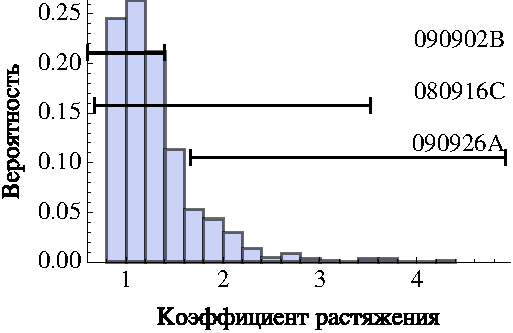
\includegraphics[width=\textwidth]{kappaDistributionHistogram}
			   			\label{fig:kappaDistributionHistogram}
			   		\end{figure}

			   		Также получены (для выбранных значений параметров):

			   		\begin{itemize}
			   			\item{Полная энергия, излученная в диапазоне $\gtrsim$ \unit[1]{ГэВ}. Результат меньше предельного значения.}
			   			\item{Доля всплесков среди наблюдаемых в диапазоне (\unit[100]{МэВ}, \unit[1]{ГэВ}), которые также можно увидеть в диапазоне (1 ГэВ, 300 ГэВ) $f_m = 0.072$. Наблюдаемое значение $f_o = 0.086$.}
			   		\end{itemize}

			   	\end{block}

			\end{column}

		\end{columns}
	\end{frame}

\end{document}